\documentclass[french]{standalone}
\usepackage{babel}
\usepackage{tkz-fct}
\usepackage{tkz-euclide}
\usepackage{color}
\usepackage{amsmath}
\usepackage{numprint}
\usepackage{amssymb}
\usepackage{amsthm}
\renewcommand*\familydefault{\sfdefault}
\usepackage{sansmath}
\sansmath
\definecolor{gray75}{gray}{0.75}
\usepackage{setspace}
	\setstretch{1.25}
\begin{document}
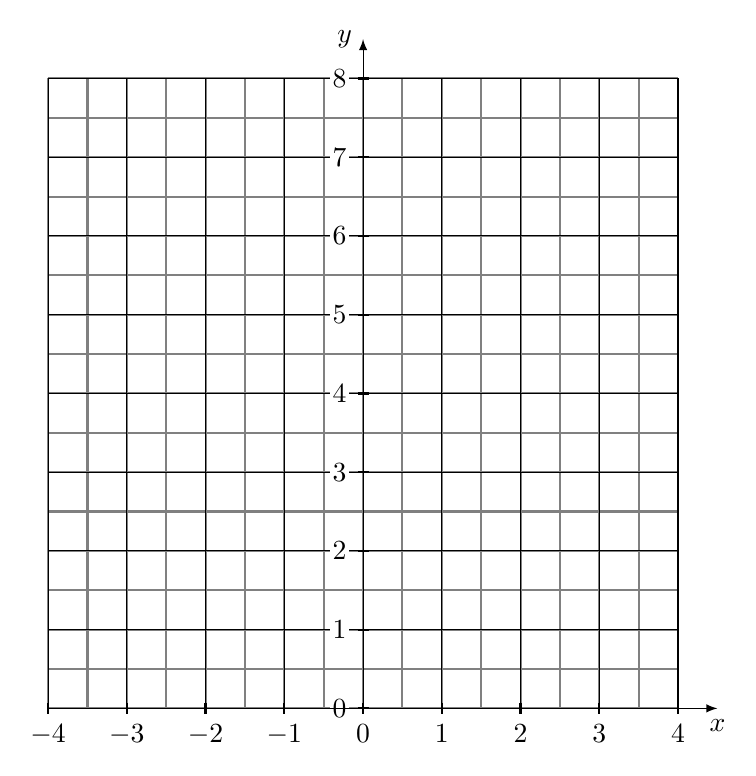
\begin{tikzpicture}
  \tkzInit[xmin=-4,xmax=4,ymin=0,ymax=8, ystep=1, xstep=1]

     \tkzGrid[color=black,sub,subxstep=0.5, subystep=0.5]
\tkzAxeY
\tkzDrawX
\tkzLabelX
\tkzFct[domain=-4:2.7,line width=2pt]{(0.5*exp(log(3)*x))}


\end{tikzpicture}
\end{document}
